\documentclass{instrukcja}
\usepackage[polish]{babel}
\usepackage[utf8]{inputenc}
\usepackage[OT4]{fontenc}

%\usepackage{dsfont}
%\usepackage[usenames,dvipsnames,svgnames,table]{xcolor}
%\usepackage[justification=centering]{caption}

\begin{document}

\materialnumber{1}
\course[MetNum]{Metody Numeryczne}
\material[Lab 1]{Instrukcja 1}
\author{B. Górecki}
%Układy równań nieliniowych
\materialtitle

\section*{Wprowadzenie}

Rozwiązanie wielu problemów inżynierskich wymaga rozwiązania układów równań nieliniowych (wśród których choć jedno równanie jest równaniem nieliniowym). Dzisiejsze laboratorium będzie poświęcone metodzie Newtona-Raphsona pozwalającej rozwiązywać takie zagadnienia. W celu przypomnienia podstawowych zagadnień zaczniemy od problemu liniowego wypływającego ze statyki mechanizmu po uwolnieniu poszczególnych członów od więzów. Umiejętność rozwiązania zagadnienia liniowego jest nieodzownym elementem implementacji metody Newtona-Raphsona.

\section{Problem liniowy}
Rozważmy mechanizm pokazany na Rysunku 1 i uwolnijmy ten układ od więzów, uwydatniając siły w parach kinematycznych. Znana jest geometria układu oraz ciężary poszczególnych członów wynoszące $G_{AB}=25$, $G_{BC}=16$ oraz $G_{CD}=53$.

\begin{figure}[h]
\centering
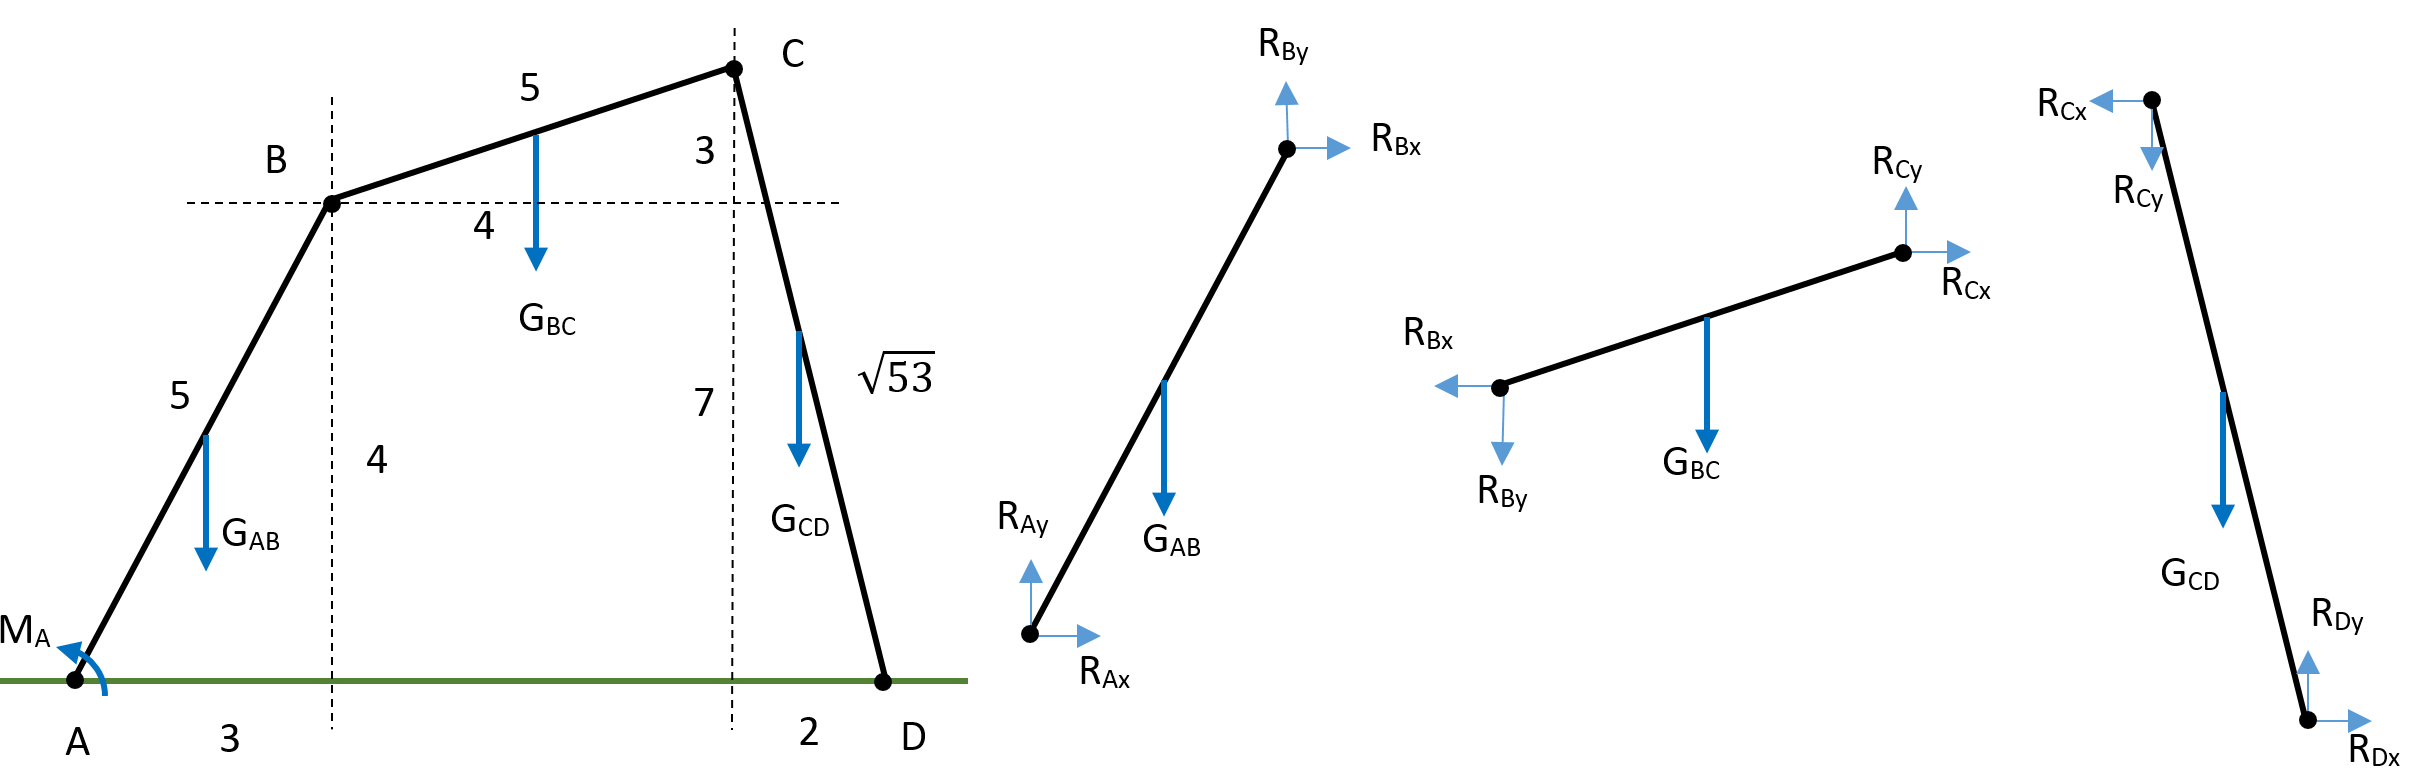
\includegraphics[width=0.9\textwidth]{mechanizm.png}
\caption[c]{Wyjściowy układ mechaniczny (po lewej) oraz poszczególne człony uwolnione od więzów (po prawej).}
\end{figure}

Dla układu o zadanej na rysunku geometrii oraz ciężarach członów podanych powyżej równania równowagi wyglądają następująco:
\begin{displaymath}
\begin{tabular}{c}
$R_{Ax}+R_{Bx} = 0$ \\
$R_{Ay}+R_{By} = G_{AB}$ \\
$M_A-1.5G_{AB}+3R_{By}-4R_{Bx}=0$ \\
$-R_{Bx}+R_{Cx}=0$ \\
$-R_{By}+R_{Cy}=G_{BC}$ \\
$-2G_{BC}-3R_{Cx}+4R_{Cy}=0$ \\
$-R_{Cx}+R_{Dx}=0$ \\
$-R_{Cy}+R_{Dy}=G_{CD}$ \\
$-G_{CD}+7R_{Dx}+2R_{Dy}=0$ \\
\end{tabular}
\end{displaymath}

W postaci macierzowej układ równań zapisuje się następująco:
\begin{displaymath}
\left[ \begin{tabular}{c c c c c c c c c} 1 & 0 & 0 & 1 & 0 & 0 & 0 & 0 & 0 \\
 0 & 1 & 0 & 0 & 1 & 0 & 0 & 0 & 0 \\
 0 & 0 & 1 & -4 & 3 & 0 & 0 & 0 & 0 \\
 0 & 0 & 0 & -1 & 0 & 1 & 0 & 0 & 0 \\
 0 & 0 & 0 & 0 & -1 & 0 & 1 & 0 & 0 \\
 0 & 0 & 0 & 0 & 0 & -3 & 4 & 0 & 0 \\
 0 & 0 & 0 & 0 & 0 & -1 & 0 & 1 & 0 \\
 0 & 0 & 0 & 0 & 0 & 0 & -1 & 0 & 1 \\
 0 & 0 & 0 & 0 & 0 & 0 & 0 & 7 & 2 \\
  \end{tabular} \right]
\left[ \begin{tabular}{c} $R_{Ax}$ \\
$R_{Ay}$ \\
$M_A$ \\
$R_{Bx}$ \\
$R_{By}$ \\
$R_{Cx}$ \\
$R_{Cy}$ \\
$R_{Dx}$ \\
$R_{Dy}$ \\
\end{tabular} \right] = \left[
\begin{tabular}{c} 0 \\
25 \\
37.5 \\
0 \\
16 \\
32 \\
0 \\
53 \\
53 \\ \end{tabular} \right]
\end{displaymath}

\subsection*{Zadanie 1}
Napisz program w C, który obliczy siły i momenty przenoszone w parach kinematycznych. Do rozwiązania układu równań wykorzystaj metodę eliminacji Gaussa, której implementacja jest dostępna w pliku {\tt Gauss.h}. (Wskazówka: Funkcja {\tt void Gauss(int n, double **M, double *F, double *x)} przyjmuje podwójny wskaźnik do macierzy - z tego względu pamiętaj o zaalokowaniu dynamicznym dwuwymiarowej tablicy - tablica statyczna miałaby typ niezgodny z nagłówkiem funkcji). Sprawdź, czy otrzymujesz poprawne rozwiązanie wynoszące:
\begin{displaymath}
\left[ \begin{tabular}{c} $R_{Ax}$ \\
$R_{Ay}$ \\
$M_A$ \\
$R_{Bx}$ \\
$R_{By}$ \\
$R_{Cx}$ \\
$R_{Cy}$ \\
$R_{Dx}$ \\
$R_{Dy}$ \\
\end{tabular} \right] = \left[
\begin{tabular}{c} 8.117647 \\
		39.088235 \\
		47.294118 \\
		- 8.117647 \\
		- 14.088235 \\
		- 8.117647 \\
		1.911765 \\
		- 8.117647 \\
		54.911765 \\ \end{tabular} \right]
\end{displaymath}

\section{Problem nieliniowy}

\subsection*{Metoda Newtona-Raphsona}
Metoda Newtona Raphsona wypływa z rozwinięcia funkcji wielu zmiennych w szereg Taylora, ucięcia go po członie liniowym i zapostulowania, że nieznany przyrost argumentów ma być taki, aby funkcja miała w tym miejscu wartość zero. Zapiszmy takie rozwinięcie dla funkcji $F(\vec x)$, gdzie $\vec x = [x,y]$, a $\vec h = [h_x, h_y]$.
\begin{displaymath}
F(\vec x_0 + \vec h) = F(\vec x_0) + \frac{\partial F}{\partial x} h_x + \frac{\partial F}{\partial y} h_y + ...
\end{displaymath}
W zapisie indeksowym napiszemy dla funkcji $F_i$ (może tych funkcji być cały wektor dla $i = 1,...,n$)
\begin{displaymath}
F_i(\vec x_0 + \vec h) = F_i(\vec x_0) + \frac{\partial F_i}{\partial x_j} h_j + ...
\end{displaymath}

$\frac{\partial F_i}{\partial x_j}$ to nic innego jak macierz Jacobiego. Wiadomo, że jest to macierz kwadratowa, jako że rozwiązujemy zagadnienie mające tyle samo równań co niewiadomych. Przyrównujemy rozwinięcie do zera - pozwoli nam to wyznaczyć takie przesunięcie argumentów, że gdyby liniowe rozwinięcie funkcji wokół danego punktu było słuszne, to w jednej iteracji otrzymywalibyśmy dokładne rozwiązanie zadania. Otrzymujemy:
\begin{displaymath}
F_i(\vec x_0 + \vec h) = F_i(\vec x_0) + \frac{\partial F_i}{\partial x_j} h_j = 0
\end{displaymath}
i tym samym
\begin{displaymath}
\frac{\partial F_i}{\partial x_j} h_j = - F_i(\vec x_0)
\end{displaymath}

Proces iteracyjny dla metody Newtona-Raphsona ma następującą postać:
\begin{enumerate}
\item Wybierz przybliżenie startowe {\it $x^1$}.
\item Przypisz k = 1.
\item Wyznacz wektor $\vec h^k$, rozwiązując układ równań $\frac{\partial F_i(\vec x^k)}{\partial x_j} h_j^k = - F_i(\vec x^k)$.
\item Zaktualizuj przybliżenie rozwiązania: $\vec x^{k+1} = \vec x^k + \vec h^k$.
\item Przypisz $k = k+1$.
\item Wróc do punktu 3. i powtarzaj aż do osiągnięcia zbieżności.
\end{enumerate}

\subsection*{Zadanie 2}

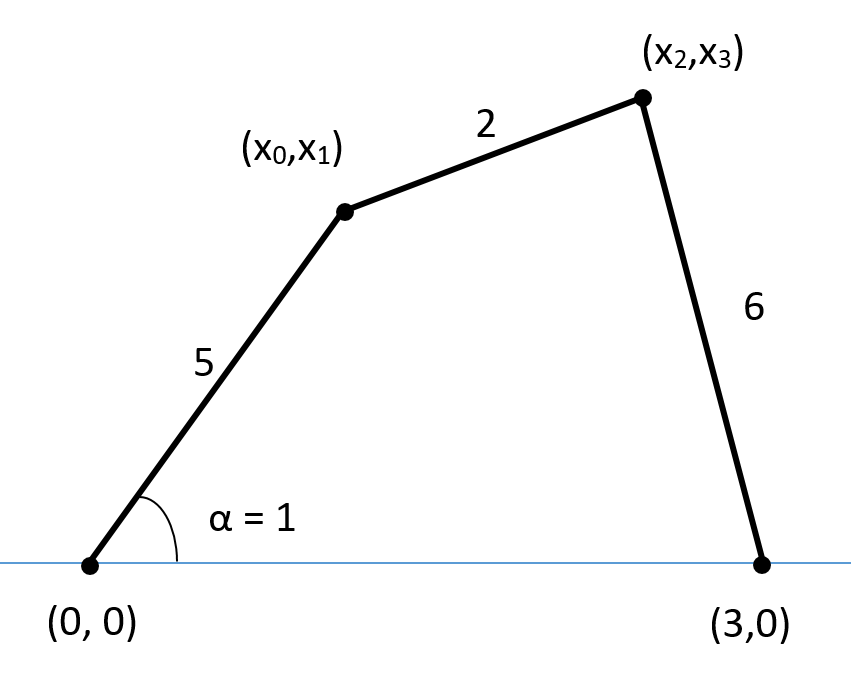
\includegraphics[width=0.5\textwidth]{czworobok.png}

Zajmijmy się teraz czworobokiem przegubowym pokazanym powyżej i rozważmy zadanie o położeniach (patrz: TMM I). Zadanie o położeniach zawsze prowadzi do układu równań nieliniowych. Do jego rozwiązania wykorzystamy metodę Newtona-Raphsona. Układ rozważymy we współrzędnych naturalnych (nieznanymi wielkościami będą współrzędne punktów $(x_0,x_1)$ i $(x_2,x_3)$, a równania więzów będą wynikać z odchylenia członu kierującego o kąt $\alpha$ od poziomu oraz długości dwóch pozostałych członów). Tym samym równania członów są postaci:
\begin{displaymath}
\begin{tabular}{c}
$x_0 = 5 \cdot cos\alpha$ \\
$x_1 = 5 \cdot sin \alpha$ \\
$(x_2-x_0)^2 + (x_3-x_1)^2 = 4$ \\
$(3-x_2)^2 + (x_3-0)^2 = 36$
\end{tabular}
\end{displaymath}
Po rozwinięciu i zapisaniu całego układu w postaci funkcji wektorowej wektorowego argumentu otrzymamy następujące sformułowanie naszego układu równań: $\vec F(\vec x) = \vec 0$, gdzie
\begin{displaymath}
\vec F(\vec x) = \left[ \begin{tabular}{c} $x_0 - 5 \cdot cos\alpha$ \\
$x_1 - 5 \cdot sin \alpha$ \\
$x_2^2-2x_0 x_2 + x_0^2 + x_3^2-2x_1 x_3 +x_1^2 -4 $ \\
$-6x_2+x_2^2+x_3^2-27$
\end{tabular} \right]
\end{displaymath}
Wyprowadziwszy powyższe równania możemy analitycznie policzyć macierz Jacobiego:
\begin{displaymath}
J = \frac{\partial \vec F}{\partial \vec x} = 
\left[ \begin{tabular}{c c c c}
1 & 0 & 0 & 0 \\
0 & 1 & 0 & 0 \\
$-2x_2+2x_0$ & $-2x_3+2x_1$ & $-2x_0+2x_2$ & $-2x_1+2x_3$ \\
0 & 0 & $-6+2x_2$ & $2x_3$ \\
\end{tabular}
\right]
\end{displaymath}

\subsection*{Zadania do wykonania}
\begin{enumerate}
\item Napisz program, który rozwiąże zadanie o położeniach przy wykorzystaniu metody Newtona-Raphsona. W tym celu stwórz następujące funkcje:
\begin{itemize}
\item {\tt void Constraints(double *x, double *F);}
\item {\tt void JacobiMatrix(double **J, double *x);}
\item {\tt void NewtonRaphson(double *x);}
\end{itemize}
\item Zmodyfikuj program tak, aby nie wymagał analitycznego obliczenia macierzy Jacobiego, ale potrafił numerycznie obliczyć tę macierz. W tym celu stwórz dodatkową funkcję {\tt void JacobiMatrixFD(double **J, double *x);} przybliżającą poprawną macierz Jacobiego macierzą obliczoną z użyciem metody różnic skończonych (ang. {\it finite difference}). Można tego dokonać z użyciem algorytmu zapisanego w poniższym pseudokodzie (metoda różnic skończonych 2-ego rzędu):

\begin{enumerate}
\item Wybierz małą wartość, np. $\epsilon = 1e-8$, stwórz wektor $\vec x'$ i $\vec x''$.
\item Pętla po wszystkich czterech kolumnach:
\begin{itemize}
\item Przypisz do $\vec x'$ i $\vec x''$ bieżącą wartość $\vec x$.
\item Zwiększ (zaburz) {\it i}-tą składową $\vec x'$ o $\epsilon$, a tę samą składową $\vec x''$ zmniejsz o $\epsilon$.
\item Wyznacz wektory wartości funkcji $\vec F (\vec x')$ oraz $\vec F (\vec x'')$.
\item Do {\it i}-tej kolumny macierzy $J$ wpisz wartości $\frac{\vec F (\vec x') - \vec F (\vec x'')}{2\epsilon}$.
\end{itemize}
\end{enumerate}

W ramach testów sprawdź, czy macierz Jacobiego dla punktu startowego obliczona metodą dokładną i numeryczną ma te same wartości. Dla punktu startowego $\vec x = [0, 5, 3, 6]$ macierz Jacobiego ma wartości
\begin{displaymath}
J = \left[ \begin{tabular}{c c c c}
1 & 0 & 0 & 0 \\
0 & 1 & 0 & 0 \\
-6 & -2 & 6 &2 \\
0 & 0 & 0 & 12 \\ \end{tabular} \right]
\end{displaymath}
\end{enumerate}
\end{document}

%W symulacjach przepływów turbulentnych z użyciem metod typu RANS wielkości turbulentne są modelowane np. przez dołączenie do równań przepływu dwóch dodatkowych równań na energię kinetyczną turbulencji oraz jej tempo dyssypacji. W rezultacie, przy zadawaniu warunków brzegowych na wlocie do obszaru, trzeba jedynie zadać profil prędkości oraz postawić warunek brzegowy dla tych dodatkowych wielkości. Np. specyfikujemy intensywność turbulencji i stosunek lepkości turbulentnej do lepkości molekularnej. Natomiast w mteodach typu LES (Large Eddy Simulation) oraz metodach hybrydowych opartych na technice LES jest to niewystarczające ze względu na fakt, że część skal turbulentnych jest jawnie rozwiązywana, tzn., że muszą istnieć w rozwiązywanym polu prędkości. Muszą zatem być te zaburzenia turbulentne obecne w profilu wlotowym.
%
%Powszechnie stosuje się trzy metody zapewnienia tego, by w symulowanym polu prędkości przepływu pojawiły się fluktuacje turbulentne. Niejednokrotnie, gdy metody typu LES lub DNS (direct numerical simulation) służą do symulacji przepływu turbulentnego w kanale, stosuje się periodyczne warunki brzegowe na wlocie i wylocie, dzięki czemu symulowany jest tak naprawdę przepływ przez nieskończenie długi kanał. W czasie takiej symulacji albo wprowadza się w sposób sztuczny delikatne zaburzenie lub polega na błędach zaokrągleń i numerycznych, które dla przepływu z odpowiednio dużą liczbą Reynoldsa stanowią wystarczające zaburzenie do zdestabilizowania przepływu i wygenerowania turbulencji. Jest to jednak metoda mało praktyczna, gdy chcemy mieć odpowiednie, zaburzone pole prędkości na wlocie do obszaru od samego początku symulacji. Zdestabilizowanie bowiem przepływu powyższą metodą bywa wcale nie takie proste. Drugą metodą jest wprowadzenie na wlocie fluktuacji uzyskanych wcześniej z poprzedzającej symulacji DNS np. przepływu w kanale. W tym celu trzeba jednak dysponować takimi danymi i poświęcić czas (również czas komputera) na wykonanie takiej symulacji dającej przepływ z odpowiednimi parametrami wielkości turbulentnych. Trzecia metoda, którą my się zajmiemy, to metoda wygenerowania syntetycznej (sztucznej) turbulencji na wlocie. Wymaga ona jedynie podania kilku parametrów określających turbulencję i generuje losowe pole zaburzeń prędkości, które spełnia podstawowe założenia zarówno równań przepływowych, jak też fizykę zjawiska turbulencji.
%
%\section{Sformułowanie teoretyczne}
%Idea metody generacji syntetycznych fluktuacji turbulentnych jest bardzo prosta. Zasadza się na następujących założeniach:
%\begin{enumerate}
%\item Każdą funkcję lub pole (np. pole prędkości) da się przedstawić za pomocą szeregu Fouriera. Można więc fluktuacje turbulentne zadać szeregiem Fouriera składającym się z odpowiednio wielu wyrazów o wielu różnych długościach fali. Te długości fali w sensie przestrzennym będą odpowiadać różnym wymiarom liniowym tworów turbulentnych.
%\item W sformułowaniu każdego z wyrazów szeregu Fouriera występuje wektor falowy, kąt przesunięcia fazowego oraz wersor określający kierunek wektora prędkości tego zaburzenia. Wielkości te będą generowane w sposób losowy.
%\item Przy powyższym losowaniu (zakładamy, że turbulencja ma charakter niedeterministyczny) należy tylko zadbać o to, by wytworzyć turbulencję o takiej intensywności, jaką zadajemy na wlocie do obszaru, aby zaburzenia o poszczególnych długościach fali odzwierciedlały fizyczny rozkład gęstości energii w funkcji liczby falowej (widmo Karmana, hipoteza K41) oraz dodatkowo spełniały równania przepływu (równanie ciągłości, a zatem warunek bezdywergentności pola prędkości, a zatem pola wygenerowanych zaburzeń).
%\item W ten sposób generujemy odpowiednio wiele niezależnych losowych pól zaburzeń (tyle, ile będzie kroków czasowych w naszej symulacji). Oczywiście w fizycznej turbulencji pole prędkości w nowej chwili jest zależne od tego, co działo się przed chwilą, toteż na koniec między niezależnymi polami wprowadzamy odpowiednią korelację w czasie, która zapewni płynność zmian w czasie.
%\end{enumerate}
%Prześledźmy teraz powoli na wzorach sposób, w jaki generuje się syntetyczną turbulencję. Określamy ogólną postać syntetycznego pola prędkości jako
%\begin{displaymath}
%\vec{v}'(\vec x) = 2 \sum_{n=1}^N{\hat{\vec u}^n cos(\vec{\kappa}^n \cdot \vec x + \psi^n) {\vec{\sigma}}^n}
%\end{displaymath}
%gdzie $\hat u^n$, $\vec{\kappa}^n$, $\psi^n$, $\vec{\sigma}^n$ oznaczają odpowiednio amplitudę, wektor falowy i przesunięcie fazowe oraz wersor kierunku n-tego modu Fouriera. Następnie trzeba określić największą i najmniejszą liczbę falową (czyli najmniejszą i największą długość fali), jakie będą obecne w generowanym spektrum. Z rozdzielczości siatki obliczeniowej (spostrzeżenia, że nie da się jednego sinusa reprezentować na mniej niż dwóch oczkach siatki) wynika, że maksymalna sensowna dla nas liczba falowa wynosi
%\begin{displaymath}
%\kappa_{max}=\frac{2 \pi}{2 \Delta}
%\end{displaymath}
%gdzie $\Delta$ oznacza wielkość oczka siatki. Najmniejszą liczbę falową zaś definiujemy jako
%\begin{displaymath}
%\kappa_1=\frac{\kappa_e}{p}
%\end{displaymath}
%gdzie $\kappa_e$ to liczba falowa związana z najbardziej energetycznymi falami ze spektrum von Karmana, a to współczynnik powinien być większy od jedności, aby w spektrum były obecne mody o długości fali większej od długości fali najbardziej energetycznych modów. Dobrą wartością jest $p=2$. Długość fali odpowiadającej modom niosącym największą energię można określić ze wzoru
%\begin{displaymath}
%\kappa_e=\frac{\alpha 9 \pi}{55 L_t}
%\end{displaymath}
%gdzie $\alpha=1.453$, a turbulentna skala długości może być określona tak samo jak w symulacjach RANS jako jedna dziesiąta grubości warstwy przyściennej.
%Kolejnym krokiem na drodze do generacji syntetycznej turbulencji jest podzielenie całego zakresu liczb falowych na $N$ modów rozłożonych równomiernie, każdy o wielkości $\Delta \kappa$. Ze wzoru na spektrum von Karmana możemy określić amplitudę każdego z modów jako
%\begin{displaymath}
%\hat{u}=(E(\kappa)\Delta \kappa)^{1/2}
%\end{displaymath}
%gdzie
%\begin{displaymath}
%E(\kappa)=c_E \frac{u_{rms}^2}{\kappa_e} \frac{(\kappa / \kappa_e)^4}{[1+(\kappa / \kappa_e)^2]^{17/6}} e^{[-2(\kappa / \kappa_{\eta})]}
%\end{displaymath}
%\begin{displaymath}
%\kappa = (\kappa_i \kappa_i)^{1/2}
%\end{displaymath}
%\begin{displaymath}
%\kappa_\eta=\epsilon^{1/4} \nu^{-3/4}
%\end{displaymath}
%Współczynnik $c_E$ otrzymujemy przez scałkowanie widma energii turbulencji po wszystkich liczbach falowych
%\begin{displaymath}
%k=\int_0^\infty{E(\kappa)d\kappa}
%\end{displaymath}
%co daje
%\begin{displaymath}
%c_E=\frac{4}{\sqrt{\pi}}\frac{\Gamma(17/6)}{\Gamma(1/3)}\cong 1.453
%\end{displaymath}
%gdzie
%\begin{displaymath}
%\Gamma(z)=\int_0^{\infty}{e^{-z'}x^{z-1}dz'}
%\end{displaymath}
%Wróćmy do algorytmu. Wylosowanie kątów $\varphi$, $\psi$ oraz $\alpha$ z przedziału od $0$ do $2 \pi$ oraz $\theta$ z przedziału od $0$ do $\pi$ (patrz rysunek poniżej oraz wzory poniżej) pozwala określić zarówno składowe wektora falowego, przesunięcie fazowe oraz kierunek, jakim skierowane jest w przestrzeni dane zaburzenie prędkości. Ostateczny wzór na wektor fluktuacji w danym punkcie przestrzeni ma postać
%\begin{displaymath}
%v_1'=2 \sum_{n=1}^N{\hat{u}^n cos(\beta^n) \sigma_1}
%\end{displaymath}
%\begin{displaymath}
%v_2'=2 \sum_{n=1}^N{\hat{u}^n cos(\beta^n) \sigma_2}
%\end{displaymath}
%\begin{displaymath}
%v_3'=2 \sum_{n=1}^N{\hat{u}^n cos(\beta^n) \sigma_3}
%\end{displaymath}
%gdzie
%\begin{displaymath}
%\beta^n=k_1^n x_1 + k_2^n x_2 + k_3^n x_3
%\end{displaymath}
%W powyższym niezmiernie istotne jest, aby wektor $\vec{\sigma}$ dla danego modu był prostopadły do wektora falowego tego modu. Ten warunek gwarantuje, że tak otrzymane pole prędkości będzie na pewno polem bezdywergentnym, a więc spełniającym równanie ciągłości. I powtórzmy jednocześnie – otrzymanie samej amplitudy z widma von Karmana gwarantuje nam też, że nasza syntetycznie generowana turbulencja ma fizyczny, zgodny z prawdziwą, rozkład energii w poszczególnych długościach fali.
%
%%\begin{figure}
%%\centering
%%\includegraphics[width=0.6\textwidth]{Wektory.png}
%%\caption[c]{Określenie położeń wektorów w oparciu o wylosowane kąty (rys. z Lars Davidson, "Fluid mechanics, turbulent flow and turbulence modeling")}
%%\end{figure}
%
%To już niemal wszystko. W ten sposób jesteśmy w stanie wygenerować dowolnie dużo niezależnych od siebie pól fluktuacji turbulentnych, które spełniają stawiane wymagania. Niemniej, aby te pola stanowiły użyteczny warunek brzegowy dla symulacji, musimy wprowadzić jeszcze korelację w czasie między nimi w myśl tego, że oczywiście to, co dzieje się na wlocie do obszaru chwilę później w bardzo dużej mierze zależy od tego, co działo się przed chwilą. Tak więc gotowe fluktuacje na wlocie będą generowane jako średnia ważona pola zaburzeń z poprzedniego kroku czasowego (z odpowiednio dużą wagą) oraz nowego pola zaburzeń z inną wagą (najczęściej znacznie mniejszą ze względu na małą separację czasową). Ostatecznie pole zaburzeń $(\vec{V}')^m$ dla m-tej chwili czasowej generuje się ze wzoru
%\begin{displaymath}
%(V'_1)^m=a(V'_1)^{m-1}+b(v'_1)^m
%\end{displaymath}
%\begin{displaymath}
%(V'_2)^m=a(V'_2)^{m-1}+b(v'_2)^m
%\end{displaymath}
%\begin{displaymath}
%(V'_3)^m=a(V'_3)^{m-1}+b(v'_3)^m
%\end{displaymath}
%gdzie współczynniki określa się ze wzoru $a=exp(-\Delta t/T)$, $b=(1-a^2)^{0.5}$. oznacza tutaj skalę czasową turbulencji i tym samym korelacja w czasie (mówiąca o tym, jak mocno obecny stan jest skorelowany ze stanem sprzed czasu $\tau$ wstecz) jest równa $exp(-\tau/T)$. Na sam koniec do samych zaburzeń turbulentnych należy dodać deterministyczny profil prędkości z wlotu tak, aby otrzymać gotowy warunek brzegowy. Przedstawiają to poniższe wzory.
%\begin{displaymath}
%v_1(0, x_2, x_3, t)=V_1(x_2,x_3)+V_1'(x_2,x_3,t)
%\end{displaymath}
%\begin{displaymath}
%v_2(0, x_2, x_3, t)=V_2(x_2,x_3)+V_2'(x_2,x_3,t)
%\end{displaymath}
%\begin{displaymath}
%v_3(0, x_2, x_3, t)=V_3(x_2,x_3)+V_3'(x_2,x_3,t)
%\end{displaymath}
%\section{Zadania}
%Otwórz w programie Microsoft Visual Studio dostarczony projekt z kodem źródłowym programu do generowania syntetycznej turbulencji na wlocie do obszaru obliczeniowego. Prześledźmy teraz wspólnie uważnie cały kod, zwracając uwagę na częste w kodzie komentarze.
%Zwróć szczególną uwagę na linie od 298 do 350. Znajdują się tam wykomentowane linie rozpoczynające się od słowa {\tt//Uzupełnij:}. Twoim zadaniem będzie wypełnić te linie poprawnym kodem źródłowym i wykonać poniższe ćwiczenia.
%\subsection*{Ćwiczenie 1}
%\begin{itemize}
%\item Korzystając z funkcji Wykres, wyświetl na ekranie spektrum energii turbulencji von Karmana. Osie odciętych i rzędnych niech będą wyskalowane liniowo.
%\item Wykomentuj kod tworzący powyższy wykres i obejrzyj to samo widmo w skali podwójnie logarytmicznej.
%\end{itemize}
%
%\subsection*{Ćwiczenie 2}
%\begin{itemize}
%\item Wykomentuj całość kodu związanego z Ćwiczeniem 1.
%\item Wyświetl na ekranie wykres przedstawiający jedną realizację losowego pola fluktuacji turbulentnych. Zwróć uwagę na linię 266 w kodzie źródłowym, która pozwala ci na łatwe zapisanie do tablic $u$, $v$, $w$ jednej z realizacji.
%\item Zmień kilka razy liczbę modów {\it nmodes} od bardzo małych (rzędu 3-5) do kilkuset. Czy zauważasz jakieś różnice w charakterze generowanych zaburzeń?
%\item Tym razem zmień wartość parametru $qm$ (zarówno w dół, jak i w górę). Uruchom kilkukrotnie program, oglądając przy tym wykres generowanych zaburzeń. Czy na skali osi rzędnych zauważasz jakieś zmiany?
%\item Na koniec zmień zdefiniowaną w parametrach grubość warstwy przyściennej $delta$. Sprawdź kilka różnych wartości, wyświetl wykresy i przyjrzyj się charakterowi generowanych fluktuacji.
%\end{itemize}
%
%\subsection*{Ćwiczenie 3}
%\begin{itemize}
%\item Uzupełnij w kodzie programu linijki, które pozwolą skorelować w czasie niezależne od siebie realizacje pól zaburzeń w całą historię fluktuacji turbulentnych, jakie można jako gotowy warunek dodać do deterministycznego profilu prędkości na wlocie.
%\item Otwórz programem Excel dwa pliki z wygenerowanymi fluktuacjami (plik z korelacją w czasie i bez korelacji w czasie). Dla kilku różnych okresów separacji w czasie wykreśl, korzystając z Excela przebieg autokorelacji danej składowej prędkości w wybranym punkcie w przestrzeni. O definicję autokorelacji zapytaj prowadzącego.
%\item W Excelu dla jednej chwili czasowej wygeneruj ostateczne pole prędkości, które można w symulacji zadać jako warunek brzegowy na wlocie, czyli taki, który zawiera zarówno deterministyczny profil prędkości, jak też losowe pole zaburzeń dla danej chwili czasu.
%\end{itemize}
%
%\section{Rozwiązanie}
%\begin{verbatim}
%// CWICZENIA
%//////////////////////////////////////////////////////////////////////////////////
%// Ad. 1. Obejrzyj spektrum von Karmana
%double *spektrum, *logomega;
%spektrum = new double[nmodes];
%logomega = new double[nmodes];
%for(int i = 0; i<nmodes; ++i)
%{
%   spektrum[i] = amp/wnre*pow(wnr[i]/wnre,4.0)/(pow(1+pow(wnr[i]/wnre,2.0),17./6.))
%                                                *exp(-2*pow(wnr[i]/wnreta,2.0));
%}
%Wykres(wnr, spektrum, nmodes, "Omega", "Spektrum");
%for(int i = 0; i<nmodes; i++)
%{
%   logomega[i] = log(wnr[i]);
%   spektrum[i] = log(amp/wnre*pow(wnr[i]/wnre,4.0)/(pow(1+pow(wnr[i]/wnre,2.0),17./6.))
%                                                *exp(-2*pow(wnr[i]/wnreta,2.0)));
%}
%Wykres(logomega, spektrum, nmodes, "ln Omega", "ln Spektrum");
%delete [] spektrum;
%delete [] logomega;
%/////////////////////////////////////////////////////////////////////////////////
%// Ad. 2. Przyjrzyj się jednej realizacji dla różnych parametrów
%// Obejrzyjmy realizacje zapisana w tablicach u, v, w
%Wykres(z, u, nz-1, "z", "u_prim");
%/////////////////////////////////////////////////////////////////////////////////
%// Ad. 3. Stworz korelacje w czasie
%double a, b;
%double dt = 0.01;
%double T = 1;
%for(int m = 1; m<nstep; ++m)
%{
%   a = exp(-dt/T);
%   b = sqrt(1-a*a);
%   for(int k = 0; k<nz-1; ++k)
%   {
%      ut[k][m] = a*ut[k][m-1] + b*ut[k][m];
%      vt[k][m] = a*vt[k][m-1] + b*vt[k][m];
%      wt[k][m] = a*wt[k][m-1] + b*wt[k][m];
%   }
%}
%/////////////////////////////////////////////////////////////////////////////////
%\end{verbatim}

